% !TeX program = xelatex
% !BIB program = biber
% !TeX TXS-program:compile = txs:///xelatex
% !TeX TXS-program:bibliography = txs:///biber
% برای خروجی کامل از build.bat / build.sh یا latexmk -xelatex main.tex استفاده کنید.
% قالب پروژه کارشناسی دانشگاه بناب
\documentclass[12pt,a4paper,oneside,fleqn]{report}

% بسته‌های پایه و صفحه‌آرایی
\usepackage{iftex}
\ifXeTeX\else
  \PackageError{BonabTemplate}{This template must be compiled with XeLaTeX}{Select XeLaTeX as the compiler.}
\fi

\usepackage[
  a4paper,
  top=2.5cm,
  bottom=2.5cm,
  left=2.5cm,
  right=2.5cm,
  footskip=1.25cm
]{geometry}

\usepackage{graphicx}
\graphicspath{{assets/}{figures/}}
\usepackage{float}
\usepackage{booktabs}
\usepackage{array}
\usepackage{longtable}
\usepackage{makecell}
\usepackage{multirow}
\usepackage{caption}
\usepackage{subcaption}
\usepackage{amsmath,amssymb,amsthm,mathtools,bm}
\usepackage{setspace}
\usepackage{enumitem}
\usepackage{etoolbox}
\usepackage{xcolor}
\usepackage{listings}
\usepackage{upquote}
\usepackage{titlesec}
\usepackage{tikz}
\usetikzlibrary{arrows.meta,positioning,shapes.geometric,fit}

% مدیریت منابع به سبک IEEE
\usepackage{csquotes}
\usepackage[
  backend=biber,
  style=ieee,
  sorting=none,
  giveninits=true,
  maxbibnames=99,
  doi=true,
  url=true,
  isbn=false
]{biblatex}
\addbibresource{references.bib}

% پیوندهای PDF؛ برای چاپ، پیوندها بدون رنگ و کادر هستند.
\usepackage[
  unicode=true,
  hidelinks,
  pdfencoding=auto
]{hyperref}
\usepackage{bookmark}

% زی‌پرشین باید پس از بیشتر بسته‌ها فراخوانی شود.
\usepackage{xepersian}

% =========================================================
% اطلاعات پروژه: برای پروژه خود فقط این فایل را ویرایش کنید.
% =========================================================

\newcommand{\UniversityNameFa}{دانشگاه بناب}
\newcommand{\MinistryNameFa}{وزارت علوم، تحقیقات و فناوری}
\newcommand{\FacultyNameFa}{دانشکده علوم پایه}
\newcommand{\DepartmentNameFa}{گروه ریاضی و علوم کامپیوتر}
\newcommand{\DegreeNameFa}{کارشناسی}
\newcommand{\FieldNameFa}{علوم کامپیوتر}
\newcommand{\OrientationFa}{عمومی}

\newcommand{\ProjectTitleFa}{کاربرد شبکه‌های عصبی فیزیک‌آگاه در ریزشبکه‌ها}
\newcommand{\StudentNameFa}{محمد امیر بابازاد}
\newcommand{\StudentNumber}{1402135104}
\newcommand{\SupervisorNameFa}{دکتر بابک آذرنوید}
\newcommand{\AdvisorNameFa}{} % در صورت نداشتن استاد مشاور، خالی بماند.
\newcommand{\AcademicYearFa}{۱۴۰۵ تا ۱۴۰۶}
\newcommand{\DefenseDateFa}{شهریور ۱۴۰۵}

\newcommand{\UniversityNameEn}{University of Bonab}
\newcommand{\FacultyNameEn}{Faculty of Basic Sciences}
\newcommand{\DepartmentNameEn}{Department of Mathematics and Computer Science}
\newcommand{\DegreeNameEn}{Bachelor of Science}
\newcommand{\FieldNameEn}{Computer Science}
\newcommand{\ProjectTitleEn}{Applications of Physics-Informed Neural Networks in Microgrids}
\newcommand{\StudentNameEn}{Muhammad Amir Babazad}
\newcommand{\SupervisorNameEn}{Dr. Babak Azarnavid}
\newcommand{\AdvisorNameEn}{}
\newcommand{\DefenseDateEn}{September 2026}

% کلیدواژه‌ها
\newcommand{\KeywordsFa}{شبکه عصبی فیزیک‌آگاه، ریزشبکه، مدیریت انرژی، یادگیری عمیق، پای‌تورچ}
\newcommand{\KeywordsEn}{Physics-informed neural network, microgrid, energy management, deep learning, PyTorch}

% فعال یا غیرفعال کردن بخش‌های اختیاری
% برای حذف هر بخش، true را به false تغییر دهید.
\newif\ifIncludeDedication
\IncludeDedicationtrue
\newif\ifIncludeAcknowledgements
\IncludeAcknowledgementstrue
\newif\ifIncludeSymbols
\IncludeSymbolstrue
\newif\ifIncludeListOfFigures
\IncludeListOfFigurestrue
\newif\ifIncludeListOfTables
\IncludeListOfTablestrue
\newif\ifIncludeListOfListings
\IncludeListOfListingstrue
\newif\ifIncludeAppendix
\IncludeAppendixfalse
\newif\ifIncludeEnglishPages
\IncludeEnglishPagestrue

% =========================================================
% تنظیم قلم‌ها
% برای تغییر قلم‌ها فقط همین فایل را ویرایش کنید.
% قلم‌های رسمی در اولویت‌اند و در نبود آن‌ها قلم آزاد جایگزین می‌شود.
% =========================================================

\IfFontExistsTF{B Mitra}{%
  \settextfont[Scale=1.05,AutoFakeBold=2]{B Mitra}
}{%
  \IfFontExistsTF{Amiri}{%
    \settextfont[Scale=1.00]{Amiri}
  }{%
    \settextfont{FreeSerif}
  }
}

% B Mitra همه نویسه‌های ریاضی فارسی (از جمله U+066A) را ندارد؛ بنابراین
% قلم ارقام و نمادهای ریاضی مستقل و از یک قلم کامل انتخاب می‌شود.
\IfFontExistsTF{Amiri}{%
  \setdigitfont{Amiri}
}{%
  \IfFontExistsTF{FreeSerif}{%
    \setdigitfont{FreeSerif}
  }{%
    \setdigitfont{DejaVu Sans}
  }
}

\IfFontExistsTF{B Nazanin}{%
  \defpersianfont\HeadingFont[Scale=1.05,AutoFakeBold=2,AutoFakeSlant=0.15]{B Nazanin}
}{%
  \IfFontExistsTF{Amiri}{%
    \defpersianfont\HeadingFont[AutoFakeBold=2,AutoFakeSlant=0.15]{Amiri}
  }{%
    \defpersianfont\HeadingFont[AutoFakeBold=2,AutoFakeSlant=0.15]{FreeSerif}
  }
}

\IfFontExistsTF{B Titr}{%
  \defpersianfont\TitleFont[Scale=1.00,AutoFakeBold=2]{B Titr}
}{%
  \IfFontExistsTF{Amiri}{%
    \defpersianfont\TitleFont[Scale=1.00,AutoFakeBold=2]{Amiri}
  }{%
    \defpersianfont\TitleFont[AutoFakeBold=2]{FreeSerif}
  }
}

\IfFontExistsTF{Times New Roman}{%
  \setlatintextfont{Times New Roman}
}{%
  \setlatintextfont{TeX Gyre Termes}
}


% نقش: صفحه‌آرایی، عنوان‌ها، فهرست‌ها، قضیه‌ها، کد و نمودار.
% محتوای علمی پروژه را اینجا ننویسید.

% متن ۱۴ پوینت با فاصلهٔ خط ۱٫۵ (پایه ۲۱ پوینت) مطابق دستورالعمل دانشگاه
\AtBeginDocument{\fontsize{14pt}{21pt}\selectfont}
\setlength{\parindent}{1.25cm}
\setlength{\parskip}{0pt}
\setlength{\emergencystretch}{2em}
\raggedbottom

% شماره صفحه وسط پایین؛ fancyhdr با bidi تداخل می‌سازد.
\pagestyle{plain}

\titleformat{\chapter}[display]
  {\centering\TitleFont\bfseries\fontsize{16pt}{24pt}\selectfont}
  {فصل \thechapter}
  {0.5em}
  {}
\titleformat{name=\chapter,numberless}[display]
  {\centering\TitleFont\bfseries\fontsize{16pt}{24pt}\selectfont}
  {}
  {0pt}
  {}
\titlespacing*{\chapter}{0pt}{-10pt}{28pt}

\titleformat{\section}
  {\HeadingFont\bfseries\itshape\fontsize{14pt}{21pt}\selectfont}
  {\thesection}
  {0.75em}
  {}
\titlespacing*{\section}{0pt}{21pt}{7pt}

\titleformat{\subsection}
  {\HeadingFont\bfseries\itshape\fontsize{14pt}{21pt}\selectfont}
  {\thesubsection}
  {0.75em}
  {}
\titlespacing*{\subsection}{0pt}{14pt}{5pt}

\titleformat{\subsubsection}
  {\HeadingFont\bfseries\fontsize{13pt}{19pt}\selectfont}
  {\thesubsubsection}
  {0.75em}
  {}

% جداکنندهٔ شمارهٔ فصل‌محور مطابق دستورالعمل دانشگاه
\SepMark{-}

% رابطه از چپ و شماره از راست (کلاس fleqn)
\setlength{\mathindent}{0pt}

\DeclareCaptionFont{bonabcaption}{\fontsize{10pt}{15pt}\selectfont}
\captionsetup{
  font={bonabcaption,stretch=1.15},
  labelfont=bf,
  justification=centering,
  singlelinecheck=false,
  labelsep=period
}
\captionsetup[table]{position=top,skip=7pt}
\captionsetup[figure]{position=bottom,skip=7pt}

% گلوله از قلم ریاضی؛ B Mitra نویسهٔ bullet ندارد.
\setlist[itemize]{label={\ensuremath{\bullet}},topsep=4pt,itemsep=2pt,parsep=0pt}
\setlist[enumerate]{topsep=4pt,itemsep=2pt,parsep=0pt}

\theoremstyle{definition}
\newtheorem{definition}{تعریف}[chapter]
\newtheorem{example}[definition]{مثال}
\theoremstyle{plain}
\newtheorem{theorem}[definition]{قضیه}
\newtheorem{lemma}[definition]{لم}
\newtheorem{proposition}[definition]{گزاره}
\theoremstyle{remark}
\newtheorem{remark}[definition]{ملاحظه}
\renewcommand{\proofname}{برهان}

\definecolor{codebg}{RGB}{247,248,250}
\definecolor{codecomment}{RGB}{45,125,70}
\definecolor{codekeyword}{RGB}{25,65,150}
\definecolor{codestring}{RGB}{160,65,45}
\renewcommand{\lstlistingname}{{\HeadingFont کد}}
\renewcommand{\lstlistlistingname}{فهرست کدها}
\lstdefinestyle{bonabcode}{
  basicstyle=\ttfamily\footnotesize,
  keywordstyle=\color{codekeyword}\bfseries,
  commentstyle=\color{codecomment},
  stringstyle=\color{codestring},
  backgroundcolor=\color{codebg},
  frame=single,
  rulecolor=\color{black!20},
  numbers=left,
  numberstyle=\tiny\color{black!55},
  numbersep=8pt,
  showstringspaces=false,
  breaklines=true,
  tabsize=4,
  captionpos=b,
  xleftmargin=1.5em,
  framexleftmargin=1.2em
}
\lstdefinestyle{bonabpython}{style=bonabcode,language=Python}
\lstset{style=bonabpython}

% سبک‌های کمکی نمودار؛ در فصل‌ها با نام tikzstyle استفاده شوند.
\tikzset{
  block/.style={draw,rounded corners,minimum width=3.2cm,minimum height=1.05cm,align=center,fill=blue!5},
  loss/.style={draw,rounded corners,minimum width=3.2cm,minimum height=1.05cm,align=center,fill=orange!10},
  flow/.style={-{Latex[length=2.5mm]},thick}
}


\begin{document}
\ApplyBonabNumbering

% دو صفحه نخست شماره نمایان و لنگر PDF ندارند.
\hypersetup{pageanchor=false}
\pagenumbering{gobble}
\thispagestyle{empty}
\vspace*{0.28\textheight}
\begin{center}
  {\TitleFont\bfseries\fontsize{20pt}{30pt}\selectfont
  بسم الله الرحمن الرحیم}
\end{center}
\vfill

\thispagestyle{empty}
\begin{center}
  
\includegraphics[width=3.2cm]{logo.pdf}

  \vspace{0.4cm}
  {\HeadingFont\bfseries\fontsize{13pt}{20pt}\selectfont
  \MinistryNameFa\\[0.25cm]
  \UniversityNameFa\\[0.25cm]
  \FacultyNameFa\\[0.15cm]
  \DepartmentNameFa}

  \vfill
  {\HeadingFont\bfseries\fontsize{15pt}{23pt}\selectfont
  پروژه \DegreeNameFa{} رشته \FieldNameFa{}، گرایش \OrientationFa{} با عنوان}

  \vspace{0.7cm}
  {\TitleFont\bfseries\fontsize{20pt}{30pt}\selectfont
  \ProjectTitleFa}

  \vfill
  {\HeadingFont\bfseries\fontsize{14pt}{21pt}\selectfont
  \SupervisorLabelFa}\\[0.25cm]
  {\fontsize{14pt}{21pt}\selectfont \SupervisorNameFa}

  \ifdefempty{\AdvisorNameFa}{}{%
    \vspace{0.5cm}
    {\HeadingFont\bfseries\fontsize{14pt}{21pt}\selectfont \AdvisorLabelFa}\\[0.25cm]
    {\fontsize{14pt}{21pt}\selectfont \AdvisorNameFa}
  }

  \vfill
  {\HeadingFont\bfseries\fontsize{14pt}{21pt}\selectfont \AuthorLabelFa}\\[0.25cm]
  {\fontsize{14pt}{21pt}\selectfont \StudentNameFa}\\[0.15cm]
  {\fontsize{12pt}{18pt}\selectfont \StudentIdLabelFa: \StudentNumber}

  \vfill
  {\HeadingFont\bfseries\fontsize{13pt}{20pt}\selectfont
  \DefenseDateFa\\[0.15cm]
  \AcademicYearLabelFa{} \AcademicYearFa}
\end{center}


% صفحات مقدماتی با شماره‌گذاری حرفی فارسی
\preliminarynumbering
\ifIncludeDedication
  % تقدیم — با \IncludeDedicationfalse در metadata حذف می‌شود.
\unnumberedchapter{تقدیم}

تقدیم به پدر و مادرم.
\vfill

\fi
\ifIncludeAcknowledgements
  % سپاسگزاری — با \IncludeAcknowledgementsfalse در metadata حذف می‌شود.
\unnumberedchapter{سپاسگزاری}

از استاد راهنما، دکتر بابک آذرنوید، که در طول انجام تحقیق راهنمایی فرمودند، قدردانی می‌شود. از گروه ریاضی و علوم کامپیوتر دانشگاه بناب نیز سپاسگزاری می‌گردد. مسئولیت کاستی‌های احتمالی بر عهده نگارنده است.
\vfill

\fi
\unnumberedchapter{چکیده}

موضوع این پروژه مدیریت انرژی یک خانه متصل به شبکه است: بار محلی، فتوولتائیک، باتری و یک نقطه تبادل با شبکه. اگر شبکه عصبی توان شبکه، شارژ، دشارژ و وضعیت شارژ را جداگانه بدهد، حتی با خطای کم ممکن است فرمان غیرقابل اجرا شود؛ مثلاً شارژ و دشارژ هم‌زمان یا وضعیت شارژ خارج از بازه. مدل پیشنهادی فقط یک فرمان علامت‌دار باتری را می‌آموزد. بقیه کمیت‌ها از یک لایه فیزیکی ثابت به‌دست می‌آیند تا توازن توان، حدود وضعیت شارژ، سقف توان باتری و نامنفی بودن توان‌ها برقرار بماند.

آزمایش ۳۲۸۹ ساعت است، از ۱۷:۰۰ روز ۱۱ ژانویه تا ۱۷:۰۰ روز ۲۷ مه ۲۰۱۶. تقویم از مجموعه مصرف وسایل \pcite{candanedo2017energy,candanedo2017uci} گرفته شده. در این اجرا فایل \lr{UCI} و \lr{NASA POWER} در دسترس نبود \pcite{nasa2016power}؛ بنابراین بار و تابش برای \lr{Stambruges} با مدل مسکونی و پوش ارتفاع خورشید ساخته شد. برنامه مرجع از برنامه‌ریزی پویا است. دو شبکه با برش زمانی ۶۰، ۲۰ و ۲۰ درصد و پنج بذر آموزش دیدند و آزمون به‌صورت بازگشتی روی وضعیت شارژ خود مدل انجام شد.

در مدل فیزیک‌تعبیه‌شده باقیمانده توازن و نرخ نقض قیود تعریف‌شده در محاسبه شناور صفر شد. مدل داده‌محور خام نزدیک‌تر به برچسب بود، اما حدود $11{.}4$ درصد وضعیت شارژ نامعتبر و $35{.}4$ درصد شارژ و دشارژ هم‌زمان داشت. هزینه مدل پیشنهادی $42{.}418 \pm 0{.}511$ شد: حدود $6{.}2$ درصد کمتر از بدون باتری و $2{.}8$ درصد بیشتر از مرجع پویا. بعد از نگاشت ایمنی، مدل داده‌محور $42{.}234 \pm 0{.}318$ گرفت؛ با پنج بذر نمی‌توان گفت کدام بهتر است. این اعداد برای همین مطالعه خانگی و ترکیبی‌اند.

\vspace{0.6cm}
\noindent\textbf{واژه‌های کلیدی:} \KeywordsFa

\ifIncludeSymbols
  \unnumberedchapter{فهرست علائم و اختصارات}

نمادها به ترتیبی آمده‌اند که در متن ظاهر می‌شوند. توان‌ها بر حسب کیلووات، انرژی باتری بر حسب کیلووات‌ساعت و گام زمان برابر یک ساعت است.

\begin{table}[H]
  \centering
  \caption*{الف) کمیت‌های سامانه}
  \begin{tabular}{>{\centering\arraybackslash}p{0.28\textwidth} p{0.60\textwidth}}
    \toprule
    \textbf{نماد} & \textbf{معنی} \\
    \midrule
    $t$ & شماره گام زمانی \\
    $P_{\mathrm{L}}(t)$ & توان مصرفی بار \\
    $P_{\mathrm{PV}}(t)$ & توان تولیدی فتوولتائیک \\
    $P_{\mathrm{G}}(t)$ & توان خالص شبکه؛ مثبت برای خرید و منفی برای فروش \\
    $P_{\mathrm{c}}(t)$ & توان شارژ باتری، نامنفی \\
    $P_{\mathrm{d}}(t)$ & توان دشارژ باتری، نامنفی \\
    $u(t)$ & فرمان علامت‌دار باتری؛ مثبت شارژ و منفی دشارژ \\
    $u_{\mathrm{safe}}(t)$ & فرمان مدل داده‌محور پس از گیره و نگاشت ایمنی \\
    $P_{\max}$ & سقف توان شارژ یا دشارژ باتری \\
    $s(t)$ & وضعیت شارژ باتری؛ نسبت انرژی ذخیره‌شده به ظرفیت نامی، در بهره‌برداری بین $s_{\min}$ و $s_{\max}$ \\
    $s_{\min},\,s_{\max}$ & کف و سقف مجاز وضعیت شارژ \\
    $E_{\max}$ & ظرفیت انرژی باتری \\
    $\eta_{\mathrm{c}},\,\eta_{\mathrm{d}}$ & بازده شارژ و دشارژ \\
    $\Delta t$ & طول گام زمان \\
    $c_{\mathrm{b}}(t),\,c_{\mathrm{s}}(t)$ & قیمت خرید و فروش برق \\
    $\kappa$ & ضریب هزینه عبور انرژی از باتری \\
    $g_{t}$ & هزینه بهره‌برداری یک گام زمانی \\
    $[z]_{+}$ & بخش مثبت $z$، برابر با $\max(0,z)$ \\
    \bottomrule
  \end{tabular}
\end{table}

\begin{table}[H]
  \centering
  \caption*{ب) کمیت‌های یادگیری و ارزیابی}
  \begin{tabular}{>{\centering\arraybackslash}p{0.28\textwidth} p{0.60\textwidth}}
    \toprule
    \textbf{نماد} & \textbf{معنی} \\
    \midrule
    $\bm{x}(t)$ & بردار ورودی شبکه در ساعت $t$ \\
    $\bm{y}^{\star}(t)$ & خروجی مرجع برنامه‌ریزی پویا \\
    $z(t)$ & خروجی آزاد شبکه پیش از نگاشت فیزیکی \\
    $r_{\mathrm{G}}(t)$ & باقیمانده توازن توان \\
    $V_{t}(s)$ & هزینه آینده در برنامه‌ریزی پویا \\
    $\mathcal{U}(s)$ & مجموعه فرمان‌های مجاز در \lr{SOC} فعلی \\
    $\mathcal{L}_{u}$ & خطای آموزش فرمان باتری \\
    $\mathrm{MSE}_{\mathrm{comp}}$ & \lr{MSE} میانگین‌گرفته‌شده روی چهار مؤلفه خروجی \\
    \bottomrule
  \end{tabular}
\end{table}

\begin{table}[H]
  \centering
  \caption*{پ) اختصارات}
  \begin{tabular}{>{\centering\arraybackslash}p{0.28\textwidth} p{0.60\textwidth}}
    \toprule
    \textbf{اختصار} & \textbf{معنی} \\
    \midrule
    \lr{PINN} & شبکه عصبی فیزیک‌آگاه \\
    \lr{SOC} & وضعیت شارژ باتری \\
    \lr{DP} & برنامه‌ریزی پویا \\
    \lr{MSE} & میانگین مربع خطا \\
    \lr{MAE} & میانگین قدر مطلق خطا \\
    \lr{MLP} & شبکه پیش‌خور چندلایه \\
    \lr{MILP} & برنامه‌ریزی خطی آمیخته عدد صحیح \\
    \lr{MPC} & کنترل پیش‌بین مدل \\
    \lr{PV} & فتوولتائیک \\
    \bottomrule
  \end{tabular}
\end{table}

\fi

\cleardoublepage
\phantomsection
\addcontentsline{toc}{chapter}{\contentsname}
\tableofcontents

\ifIncludeListOfFigures
  \cleardoublepage
  \phantomsection
  \addcontentsline{toc}{chapter}{\listfigurename}
  \listoffigures
\fi

\ifIncludeListOfTables
  \cleardoublepage
  \phantomsection
  \addcontentsline{toc}{chapter}{\listtablename}
  \listoftables
\fi

\ifIncludeListOfListings
  \cleardoublepage
  \phantomsection
  \addcontentsline{toc}{chapter}{\lstlistlistingname}
  \lstlistoflistings
\fi

% متن اصلی از صفحه ۱ آغاز می‌شود.
\mainnumbering
\chapter{کلیات پروژه}
\label{chap:introduction}

\section{مقدمه}
گسترش منابع انرژی تجدیدپذیر و ذخیره‌سازهای الکتریکی، ساختار سنتی شبکه قدرت را به سمت سامانه‌های توزیع‌شده و هوشمند سوق داده است. ریزشبکه مجموعه‌ای از منابع تولید پراکنده، بارهای محلی و تجهیزات ذخیره‌سازی است که می‌تواند در حالت متصل به شبکه اصلی یا به‌صورت جزیره‌ای کار کند. بهره‌برداری مناسب از این اجزا به یک سامانه مدیریت انرژی نیاز دارد تا در هر بازه زمانی، میزان تولید، مصرف، شارژ یا دشارژ باتری و تبادل توان با شبکه اصلی را تعیین کند.

مدیریت انرژی ریزشبکه تنها یک مسئله پیش‌بینی نیست؛ تصمیم‌های حاصل باید محدودیت‌های فیزیکی مانند توازن توان، ظرفیت باتری، حدود توان مبدل‌ها و دامنه مجاز وضعیت شارژ را رعایت کنند. از طرف دیگر، عدم قطعیت تولید خورشیدی و تغییرات بار سبب می‌شود که مدل‌سازی دقیق سامانه دشوار باشد. روش‌های بهینه‌سازی کلاسیک می‌توانند این قیود را به‌طور صریح اعمال کنند، ولی حل مکرر آن‌ها در مسائل بزرگ یا برخط ممکن است پرهزینه باشد. روش‌های یادگیری ماشین سرعت استنتاج مناسبی دارند، اما اگر صرفاً از داده استفاده کنند، لزوماً سازگاری فیزیکی خروجی را تضمین نمی‌کنند.

شبکه‌های عصبی فیزیک‌آگاه یا \lr{PINN} روشی برای ترکیب داده و دانش پیشین فیزیکی فراهم می‌کنند. در این رویکرد، معادلات حاکم بر سامانه بخشی از تابع هزینه آموزش هستند؛ بنابراین شبکه عصبی افزون بر برازش داده، برای رعایت قوانین فیزیکی نیز آموزش می‌بیند. چارچوب عمومی این روش توسط رئیسی، پردیکاریس و کارنیاداکیس برای حل و شناسایی معادلات دیفرانسیل غیرخطی ارائه شده است \pcite{raissi2019pinns}.

در سوی دیگر، پژوهش‌های مدیریت انرژی ریزشبکه نشان می‌دهند که مدل بهره‌برداری باید هم‌زمان تبادل انرژی، سود یا هزینه مشارکت‌کنندگان و قیود تجهیزاتی را در نظر گیرد. برای نمونه، اولادجو و فولی یک مدل ریزشبکه متصل به شبکه را با تولید خورشیدی، باتری و چند مشارکت‌کننده بررسی کرده و برای تخصیص منصفانه سود از نظریه بازی و برای حل مسئله از الگوریتم بهینه‌سازی مبتنی بر آموزش و یادگیری استفاده کرده‌اند \pcite{oladejo2019microgrid}. پروژه حاضر از ترکیب ایده فیزیک‌آگاه با ساختار فیزیکی و اقتصادی مدیریت انرژی ریزشبکه الهام می‌گیرد.

\section{بیان مسئله}
یک مدل یادگیری برای مدیریت انرژی ریزشبکه، نگاشتی میان اطلاعات ورودی و تصمیم‌های بهره‌برداری ایجاد می‌کند. ورودی‌ها می‌توانند شامل زمان، تقاضای بار، توان خورشیدی، قیمت برق و وضعیت شارژ باتری باشند. خروجی‌ها نیز می‌توانند توان دریافتی از شبکه، توان شارژ و دشارژ باتری یا برنامه تبادل انرژی را نشان دهند. اگر این نگاشت تنها با کمینه‌سازی خطای داده آموزش داده شود، ممکن است خروجی مدل از نظر عددی به داده نزدیک باشد، اما معادله توازن توان یا حدود ذخیره‌ساز را نقض کند.

مسئله اصلی این پروژه آن است که چگونه می‌توان دانش فیزیکی ریزشبکه را در فرایند آموزش شبکه عصبی وارد کرد تا مدل، علاوه بر دقت داده‌ای، سازگاری فیزیکی بیشتری داشته باشد. ایده محوری آن است که باقیمانده معادلات توازن و پویایی ذخیره‌ساز در نقاط آموزش محاسبه و به تابع هزینه افزوده شود. به این ترتیب، فضای پاسخ‌های قابل قبول شبکه عصبی محدودتر می‌شود و انتظار می‌رود مدل با داده کمتر نیز رفتار معقول‌تری داشته باشد.

\section{اهمیت و ضرورت}
استفاده از مدل‌های فیزیک‌آگاه در ریزشبکه از چند جهت اهمیت دارد:
\begin{itemize}
  \item داده‌های واقعی سامانه قدرت ممکن است محدود، پرهزینه یا همراه با نویز باشند؛
  \item قوانین اصلی مانند بقای انرژی از پیش معلوم‌اند و نادیده‌گرفتن آن‌ها موجب اتلاف اطلاعات می‌شود؛
  \item در کاربردهای کنترلی، نقض قیود فیزیکی می‌تواند تصمیم تولیدشده را غیرقابل اجرا کند؛
  \item یک مدل آموزش‌دیده می‌تواند پس از آموزش، تصمیم یا تخمین را با سرعت بیشتری تولید کند؛
  \item ترکیب مدل‌محور و داده‌محور امکان بررسی تعادل میان دقت، سرعت و قابلیت اعتماد را فراهم می‌سازد.
\end{itemize}

\section{اهداف پروژه}
هدف اصلی، تدوین و پیاده‌سازی یک چارچوب اولیه برای کاربرد شبکه‌های عصبی فیزیک‌آگاه در مدیریت انرژی ریزشبکه است. اهداف فرعی عبارت‌اند از:
\begin{enumerate}
  \item مطالعه مبانی شبکه‌های عصبی فیزیک‌آگاه و مدیریت انرژی ریزشبکه؛
  \item استخراج معادلات و قیود مناسب برای یک ریزشبکه متصل به شبکه؛
  \item تعریف تابع هزینه ترکیبی شامل مؤلفه داده و مؤلفه فیزیکی؛
  \item طراحی ساختار قابل پیاده‌سازی با پایتون و پای‌تورچ؛
  \item تعریف یک روش ارزیابی برای مقایسه مدل فیزیک‌آگاه و مدل صرفاً داده‌محور؛
  \item سنجش خطای پیش‌بینی، باقیمانده فیزیکی، نقض قیود و هزینه بهره‌برداری پس از اجرای آزمایش‌ها.
\end{enumerate}

\section{پرسش‌های پروژه}
این پروژه بر پرسش‌های زیر متمرکز است:
\begin{enumerate}
  \item چگونه می‌توان معادلات توازن توان و وضعیت شارژ باتری را در تابع هزینه شبکه عصبی وارد کرد؟
  \item وزن مؤلفه‌های داده‌ای و فیزیکی تابع هزینه چه اثری بر آموزش مدل دارد؟
  \item آیا مدل فیزیک‌آگاه نسبت به مدل صرفاً داده‌محور، نقض قیود کمتری ایجاد می‌کند؟
  \item چه معیارهایی برای ارزیابی هم‌زمان دقت و سازگاری فیزیکی مناسب‌اند؟
\end{enumerate}

\section{دامنه و محدودیت‌ها}
مدل اولیه این گزارش یک ریزشبکه متصل به شبکه شامل تولید خورشیدی، باتری، بار محلی و تبادل توان با شبکه اصلی را در نظر می‌گیرد. تمرکز اصلی بر لایه مدیریت انرژی است و جزئیات الکترومغناطیسی مبدل‌ها یا پایداری گذرای شبکه در دامنه نسخه اولیه قرار نمی‌گیرد. همچنین نتایج عددی باید بر اساس داده و اجرای واقعی کد گزارش شوند و هیچ نتیجه‌ای پیش از انجام آزمایش فرض نمی‌شود.

\section{ساختار گزارش}
در فصل~\ref{chap:background} مبانی ریزشبکه، مدیریت انرژی و شبکه‌های عصبی فیزیک‌آگاه مرور می‌شود. فصل~\ref{chap:method} چارچوب پیشنهادی و تابع هزینه را توضیح می‌دهد. فصل~\ref{chap:implementation} به ساختار پیاده‌سازی و روش ارزیابی اختصاص دارد. سرانجام، فصل~\ref{chap:conclusion} جمع‌بندی و مسیرهای ادامه کار را ارائه می‌کند.

\chapter{مبانی نظری و پیشینه پژوهش}
\label{chap:background}

\section{مدل ریزشبکه متصل به شبکه}
ریزشبکه مورد مطالعه همان تعریف فصل قبل است: بار محلی، منبع فتوولتائیک، باتری و یک اتصال به شبکه بالادست. در هر گام، توان بار و تولید \lr{PV} \textbf{برون‌زاد}اند؛ یعنی از بیرون مدل می‌آیند و کنترل‌کننده آن‌ها را عوض نمی‌کند. تصمیم فقط درباره استفاده از باتری و تبادل با شبکه است. این سطح، بهره‌برداری انرژی را توصیف می‌کند و جایگزین تحلیل گذرای ولتاژ، فرکانس یا حفاظت نیست.

نمادهای گام $t$ از این قرارند
\begin{itemize}
  \item $P_{\mathrm{L}}(t)$: توان بار بر حسب کیلووات
  \item $P_{\mathrm{PV}}(t)$: توان فتوولتائیکِ در دسترس، نامنفی
  \item $P_{\mathrm{G}}(t)$: توان خالص شبکه؛ مثبت برای خرید و منفی برای فروش
  \item $P_{\mathrm{c}}(t)$ و $P_{\mathrm{d}}(t)$: توان شارژ و دشارژ باتری، هر دو نامنفی
  \item $s(t)$: وضعیت شارژ، یعنی نسبت انرژی ذخیره‌شده به ظرفیت نامی
  \item $c_{\mathrm{b}}(t)$ و $c_{\mathrm{s}}(t)$: قیمت خرید و فروش برق
\end{itemize}

نمادگذاری توان و تفکیک لایه بهره‌برداری از لایه‌های اقتصادی گسترده‌تر با مسئله ریزشبکه متصل به شبکه هم‌راستا است \pcite{oladejo2019microgrid}. با این حال، در این گزارش فقط یک بهره‌بردار و یک اتصال شبکه وجود دارد.

\section{توازن توان و دینامیک باتری}
سمت چپ رابطه زیر منابع توان (خرید از شبکه، تولید فتوولتائیک و دشارژ) و سمت راست مصارف (بار و شارژ) است
\begin{equation}
  P_{\mathrm{G}}(t)+P_{\mathrm{PV}}(t)+P_{\mathrm{d}}(t)=P_{\mathrm{L}}(t)+P_{\mathrm{c}}(t)
  \label{eq:power-balance}
\end{equation}
اگر این برابری برقرار نباشد، \textbf{باقیمانده توازن} چنین تعریف می‌شود
\begin{equation}
  r_{\mathrm{G}}(t)=P_{\mathrm{G}}(t)+P_{\mathrm{PV}}(t)+P_{\mathrm{d}}(t)-P_{\mathrm{c}}(t)-P_{\mathrm{L}}(t)
  \label{eq:power-residual}
\end{equation}
مقدار صفر برای $r_{\mathrm{G}}$ یعنی توازن برقرار است. رفتار باتری با مدل انرژی گسسته تقریب زده می‌شود
\begin{equation}
  s(t+\Delta t)=s(t)+\frac{\eta_{\mathrm{c}}P_{\mathrm{c}}(t)\Delta t}{E_{\max}}-\frac{P_{\mathrm{d}}(t)\Delta t}{\eta_{\mathrm{d}}E_{\max}}
  \label{eq:soc-dynamics}
\end{equation}
که در آن $E_{\max}$ ظرفیت انرژی بر حسب کیلووات‌ساعت، $\Delta t=1\,\mathrm{h}$ طول گام، و $\eta_{\mathrm{c}}$ و $\eta_{\mathrm{d}}$ بازده شارژ و دشارژ هستند. حدهای ایمنی عبارت‌اند از
\begin{equation}
  s_{\min}\leq s(t)\leq s_{\max},\qquad
  0\leq P_{\mathrm{c}}(t),P_{\mathrm{d}}(t)\leq P_{\max}
  \label{eq:soc-bounds}
\end{equation}
برای یک باتری تک‌مبدله، شارژ و دشارژ هم‌زمان مجاز نیست. این \textbf{قید انحصار} به صورت زیر نوشته می‌شود
\begin{equation}
  P_{\mathrm{c}}(t)P_{\mathrm{d}}(t)=0
  \label{eq:exclusivity}
\end{equation}

\section{هزینه بهره‌برداری}
هزینه یک گام از سه بخش تشکیل می‌شود: هزینه خرید از شبکه، درآمد فروش به شبکه، و یک جریمه کوچک برای عبور انرژی از باتری
\begin{equation}
  g_{t}=c_{\mathrm{b}}(t)[P_{\mathrm{G}}(t)]_{+}\Delta t
  -c_{\mathrm{s}}(t)[-P_{\mathrm{G}}(t)]_{+}\Delta t
  +\kappa\bigl(P_{\mathrm{c}}(t)+P_{\mathrm{d}}(t)\bigr)\Delta t
  \label{eq:step-cost}
\end{equation}
عملگر $[z]_{+}=\max(0,z)$ بخش مثبت است؛ بنابراین فقط وقتی $P_{\mathrm{G}}$ مثبت است هزینه خرید و فقط وقتی منفی است درآمد فروش ظاهر می‌شود. وجود $\Delta t$ یکدستی واحدهای هزینه را حفظ می‌کند و رابطه را به گام یک‌ساعته محدود نمی‌کند. در مدل حاضر، $\kappa$ نماینده‌ای ساده‌شده از استهلاک عبوری باتری است، نه مدل الکتروشیمیایی واقعی. مدل‌های بهینه‌سازی بهره‌برداری نیز معمولاً هزینه انرژی را با حدهای توان و \lr{SOC} باتری همراه می‌کنند \pcite{elhendawi2018optimal}.

\section{یادگیری فیزیک‌آگاه و قید سخت}
در چارچوب \lr{PINN} متداول، شبکه خروجی آزاد می‌دهد و باقیمانده معادلات فیزیکی به تابع آموزش افزوده می‌شود \pcite{raissi2019pinns}. مزیت آن پیوند داده و مدل است. با این حال جریمه نرم، چون ضریب محدودی دارد، به‌تنهایی تضمین نمی‌کند که خروجی نهایی دقیقاً قید را رعایت کند. در بهره‌برداری انرژی حتی نقض کوچک \lr{SOC} یا توان با علامت نامعتبر می‌تواند فرمان را غیرقابل اجرا کند.

	extbf{قید سخت} یعنی قید در خود معماری اعمال شود، نه فقط در زیان. پژوهش‌ها نشان داده‌اند لایه‌های تحلیلی یا نرافکنی می‌توانند بعضی قیود را دقیقاً تضمین کنند \pcite{lu2021hardconstraints,chen2024hardlinear}. در این کار همین ایده برای قیود جبری ریزشبکه به کار می‌رود. روش حاضر یک \lr{PINN} حل‌کننده معادله دیفرانسیل جزئی نیست؛ تعبیر دقیق‌تر آن یادگیری فیزیک‌تعبیه‌شده است: فیزیک در نگاشت خروجی نشسته است، نه فقط در جریمه.

\section{جایگاه کار در پیشینه}
\subsection{مدیریت انرژی مبتنی بر بهینه‌سازی}
روش‌های کلاسیک، بهره‌برداری را به‌صورت برنامه‌ریزی خطی یا آمیخته عدد صحیح، برنامه‌ریزی پویا، یا کنترل پیش‌بین مدل صورت‌بندی می‌کنند. 	extbf{برنامه‌ریزی پویا} تصمیم جاری را با رابطه بلمن به هزینه آینده پیوند می‌دهد \pcite{bertsekas2017dp}. 	extbf{برنامه‌ریزی خطی آمیخته عدد صحیح} (\lr{MILP}) برای تصمیم‌های گسسته مناسب است و 	extbf{کنترل پیش‌بین مدل} (\lr{MPC}) افق لغزان را بازبهینه می‌کند. مطالعات موردی ریزشبکه نشان داده‌اند که \lr{MPC/MILP} می‌تواند هزینه و قیود بهره‌برداری را در یک صورت‌بندی صریح ترکیب کند \pcite{parisio2014mpc,parisio2014experimental,elhendawi2018optimal}. این روش‌ها مرجع‌هایی تفسیرپذیر فراهم می‌کنند، اما هزینه حل آن‌ها به طول افق، تفکیک شبکه حالت، سناریوها و جزئیات مدل وابسته است. برنامه‌ریزی پویای این گزارش نیز مرجع گسسته است و ادعای بهینگی پیوسته ندارد.

\subsection{مدیریت انرژی مبتنی بر یادگیری}
یادگیری تقویتی، سیاست کنترل را از تعامل با محیط می‌آموزد و شبکه‌های عصبی نیز می‌توانند به‌صورت جانشین نظارت‌شده، نگاشت خروجی یک حل‌کننده را تقریب بزنند. مرور کاربرد یادگیری تقویتی در پاسخ‌گویی بار، ظرفیت این روش‌ها و در عین حال دشواری ارزیابی و تعمیم را نشان می‌دهد \pcite{vazquez2019rl}. در این پروژه مسیر دوم دنبال می‌شود: برچسب‌ها از برنامه‌ریزی پویا می‌آیند و شبکه با بهینه‌ساز آدام آموزش می‌بیند \pcite{kingma2015adam}. مسئله مشترک آن است که خروجی آزاد یا سیاست یادگرفته‌شده، بدون سازوکار اضافی لزوماً توازن توان، حدود \lr{SOC} و انحصار متقابل شارژ و دشارژ را رعایت نمی‌کند؛ بنابراین خطای تقلید کم به‌تنهایی گواه امکان‌پذیری نیست.

\subsection{اعمال قید در کنترل‌کننده‌های یادگرفته‌شده}
در یادگیری تقویتی ایمن، مسئله را می‌توان به‌شکل فرایند تصمیم‌گیری مارکوف مقید نوشت \pcite{altman1999cmdp} و قید را با بهینه‌سازی سیاست مقید یا توابع لیاپانوف وارد کرد \pcite{achiam2017cpo,chow2018lyapunov}. بنچمارک‌های اکتشاف ایمن نیز تأکید می‌کنند که پاداش و ایمنی باید جداگانه گزارش شوند \pcite{ray2019safexp}. روش‌های جریمه‌ای ساده‌ترند، اما رعایت قید به وزن جریمه و کیفیت آموزش وابسته می‌ماند \pcite{garcia2015survey}.

راه دیگر، محدود کردن مستقیم فضای خروجی است. \lr{OptNet} یک برنامه درجه‌دو تفکیک‌پذیر را به‌صورت لایه شبکه وارد می‌کند \pcite{amos2017optnet} و شبکه‌های محدب نسبت به ورودی، ساختاری را فراهم می‌کنند که بهینه‌سازی روی برخی ورودی‌ها محدب بماند \pcite{amos2017icnn}. معماری‌های قید سخت نیز قید را با بازنپارامتری یا لایه تحلیلی اعمال می‌کنند \pcite{lu2021hardconstraints,chen2024hardlinear}. انتخاب حاضر از این خانواده است، اما حل‌کننده بهینه‌سازی تفکیک‌پذیر یا \lr{ICNN} نیست: یک نگاشت بسته و بدون پارامتر، تنها فرمان باتری را به چهار کمیت قابل اجرا تبدیل می‌کند. این سادگی مخصوص قیود جبری مدل حاضر است و برتری عمومی نسبت به روش‌های ایمن دیگر ادعا نمی‌شود.

\subsection{یادگیری فیزیک‌آگاه در سامانه‌های انرژی}
در شبکه‌های \lr{PINN} متعارف، باقیمانده معادله دیفرانسیل در تابع آموزش ظاهر می‌شود \pcite{raissi2019pinns} و چارچوب گسترده‌تر یادگیری فیزیک‌آگاه، ورود دانش فیزیکی از راه داده، زیان یا معماری را در بر می‌گیرد \pcite{karniadakis2021piml}. با این حال، مسئله این گزارش حل یک \lr{PDE} نیست. توازن توان و گذار ساعتی باتری روابط جبری و گسسته‌اند و در لایه خروجی دقیقاً محاسبه می‌شوند، نه آن‌که باقیمانده آن‌ها فقط کمینه شود. ازاین‌رو، اصطلاح دقیق‌تر برای روش حاضر «شبکه فیزیک‌تعبیه‌شده» است؛ صفر شدن نقض‌های تعریف‌شده خاصیت طراحی این نگاشت است، نه کشف آماری. جدول~\ref{tab:approach-comparison} نقش هر رویکرد را در این گزارش، نه لزوماً در یک آزمایش چهارطرفه، خلاصه می‌کند.

\begin{table}[H]
  \centering
  \caption{مقایسه رویکردهای تولید برنامه انرژی}
  \label{tab:approach-comparison}
  \begin{tabular}{>{\centering\arraybackslash}p{0.22\textwidth}>{\centering\arraybackslash}p{0.22\textwidth}>{\centering\arraybackslash}p{0.22\textwidth}>{\centering\arraybackslash}p{0.22\textwidth}}
    \toprule
    \textbf{رویکرد} & \textbf{داده یا مدل لازم} & \textbf{وضعیت قیدها} & \textbf{نقش در این پروژه} \\
    \midrule
    برنامه‌ریزی پویا & مدل و افق برون‌زاد & مقید، تا دقت شبکه حالت & مرجع اقتصادی \\
    شبکه داده‌محور آزاد & نمونه برچسب‌دار & تضمینی ندارد & \lr{baseline} یادگیری \\
    \lr{PINN} با جریمه نرم & نمونه و باقیمانده قانون & وابسته به وزن جریمه & فقط انگیزه روش‌شناختی؛ در این گزارش آموزش داده نشد \\
    شبکه فیزیک‌تعبیه‌شده & نمونه و نگاشت فیزیکی & سخت، برای قیود مدل‌شده & مدل پیشنهادی \\
    \bottomrule
  \end{tabular}
\end{table}

\section{مرجع برنامه‌ریزی پویا}
اگر شبکه فقط هزینه همان ساعت را کمینه کند، یک قاعده 	extbf{حریصانه} می‌آموزد و آینده باتری را نمی‌بیند. برای جلوگیری از این کار، برنامه مرجع با برنامه‌ریزی پویا ساخته می‌شود. حالت برابر \lr{SOC} و فرمان برابر توان علامت‌دار باتری است. اگر $V_{t}(s)$ کمینه هزینه از زمان $t$ به بعد در وضعیت $s$ باشد، رابطه بلمن چنین است
\begin{equation}
  V_{t}(s)=\min_{u\in\mathcal{U}(s)}\bigl\{g_{t}(s,u)+V_{t+1}\bigl(f(s,u)\bigr)\bigr\}
  \label{eq:bellman}
\end{equation}
که $f$ همان دینامیک~\eqref{eq:soc-dynamics} و $\mathcal{U}(s)$ مجموعه فرمان‌های مجاز در \lr{SOC} فعلی است. در پیاده‌سازی حاضر شرط نهایی $V_{T}(s)=0$ برای همه نقاط شبکه وضعیت در نظر گرفته شده است؛ بنابراین ارزش بازیافت یا هدف نهایی جداگانه‌ای برای باتری اعمال نمی‌شود. \lr{SOC} در مرجع روی شبکه‌ای با گام $0{.}01$ گسسته می‌شود؛ بنابراین مرجع، تقریب عددیِ یک حل‌کننده افق کامل با آینده‌نگری کامل است، نه بهینه دقیق پیوسته.

\section{جمع‌بندی فصل}
این فصل قیود اصلی و شاخص هزینه را مشخص کرد. تفاوت اساسی شبکه فیزیک‌تعبیه‌شده با مدل آزاد آن است که امکان‌پذیریِ قیود مدل‌شده تنها یک معیار پس از آموزش نیست؛ بخشی از تعریف خروجی است. فصل بعد نحوه ساخت داده، معماری و آزمون بازگشتی را دقیق می‌کند.

\chapter{روش‌شناسی}
\label{chap:method}

\section{جریان کلی آزمایش}
شکل~\ref{fig:experiment-flow} جریان آزمایش را نشان می‌دهد. ابتدا از سری بار و \lr{PV}، برنامه مرجع مقید با برنامه‌ریزی پویا ساخته می‌شود. سپس دو شبکه با این داده آموزش می‌بینند. تفاوت آن دو در نحوه تعریف خروجی است: شبکه داده‌محور چهار خروجی آزاد می‌دهد، اما شبکه فیزیک‌تعبیه‌شده فقط فرمان باتری را می‌سازد و همه متغیرهای دیگر از قوانین فصل قبل حاصل می‌شوند. در انتها، هر دو مدل روی افق آزمون با \lr{SOC} تولیدشده توسط خودشان بازگشت داده می‌شوند.

\begin{figure}[H]
  \centering
  \begin{tikzpicture}[node distance=0.85cm, every node/.style={align=center}]
    \node[block, minimum width=5.4cm] (data) {داده عمومی ترکیبی\\بار، \lr{PV}، تعرفه و زمان};
    \node[block, below=of data, minimum width=5.4cm] (dp) {برنامه‌ریزی پویا\\برنامه مرجع مقید};
    \node[block, below=of dp, minimum width=5.4cm] (nets) {آموزش دو شبکه\\داده‌محور و فیزیک‌تعبیه‌شده};
    \node[loss, below=of nets, minimum width=5.4cm] (layer) {لایه فیزیکی قطعی\\توان، \lr{SOC} و توازن};
    \node[loss, below=of layer, minimum width=5.4cm, fill=yellow!8] (eval) {آزمون بازگشتی\\امکان‌پذیری و هزینه};
    \draw[flow] (data) -- (dp);
    \draw[flow] (dp) -- (nets);
    \draw[flow] (nets) -- (layer);
    \draw[flow] (layer) -- (eval);
  \end{tikzpicture}
  \caption{جریان مطالعه موردی و مقایسه کنترل‌کننده‌ها. لایه فیزیکی در مدل فیزیک‌تعبیه‌شده بخشی از خودِ خروجی است؛ برای مدل داده‌محور فقط در زنجیره ترمیم‌شده هزینه اعمال می‌شود.}
  \label{fig:experiment-flow}
\end{figure}

\section{بردار ورودی و مرجع آموزشی}
برای ساعت $t$، بردار ورودی شامل زمان تناوبی، وضعیت روز، بار، \lr{PV}، تعرفه، \lr{SOC} و پنجره پیش‌بینی کوتاه است:
\begin{equation}
\begin{split}
  \bm{x}(t)=\bigl(&\sin(2\pi h/24),\,\cos(2\pi h/24),\,d,\,P_{\mathrm{L}},\,P_{\mathrm{PV}},\,c_{\mathrm{b}},\,c_{\mathrm{s}},\,s,\\
  &P_{\mathrm{L}}^{t+1},\,P_{\mathrm{PV}}^{t+1},\,P_{\mathrm{L}}^{t+3},\,P_{\mathrm{PV}}^{t+3}\bigr).
\end{split}
  \label{eq:model-input}
\end{equation}
$h$ ساعت روز و $d$ نشانگر روز کاری است. مقادیر یک و سه ساعت آینده، پیش‌بینی بی‌خطا فرض می‌شوند. این فرض برای مقایسه آفلاین با برنامه مرجع است و ادعای دسترسی بی‌خطا به پیش‌بینی در میدان نیست.

برنامه‌ریزی پویا با مشاهده کل افق برون‌زاد، دنباله مرجع
\begin{equation}
  \bm{y}^{\star}(t)=\bigl(P_{\mathrm{G}}^{\star},\,P_{\mathrm{c}}^{\star},\,P_{\mathrm{d}}^{\star},\,s^{\star}(t+\Delta t)\bigr)
  \label{eq:reference-output}
\end{equation}
را می‌سازد. آماره‌های استانداردسازی، یعنی میانگین و انحراف معیار، فقط از مجموعه آموزش محاسبه می‌شوند تا از نشت آماری مجموعه اعتبارسنجی و آزمون جلوگیری شود.

\section{شبکه داده‌محور آزاد}
مدل نخست یک شبکه پیش‌خور با دو لایه پنهان ۳۲ واحدی و فعال‌ساز تانژانت هیپربولیک است. خروجی آن چهار مؤلفه~\eqref{eq:reference-output} را مستقیماً پیش‌بینی می‌کند. تابع آموزش آن میانگین مربع خطای خروجی استانداردشده است. این مدل برای آن در نظر گرفته شده است که نشان دهد نزدیک بودن به برچسب، به‌تنهایی معادلِ قابل‌اجرا بودن برنامه نیست.

خروجی خام برای سنجش نقض‌ها با \lr{SOC} پیش‌بینی‌شده خود مدل بازگشت داده می‌شود. در زنجیره اجرایی ترمیم‌شده، \lr{SOC} ورودی هر گام از فرمان نگاشت‌یافته و دینامیک باتری دوباره محاسبه می‌شود، نه از مؤلفه خام \lr{SOC} شبکه. برای محاسبه هزینه منصفانه، فرمان خام مدل داده‌محور با نگاشت ایمنی پس‌پردازشی
\begin{equation}
  u_{\mathrm{safe}}=\mathrm{clip}(\hat{P}_{\mathrm{c}}-\hat{P}_{\mathrm{d}},-P_{\max},P_{\max})
  \label{eq:usafe}
\end{equation}
به لایه~\eqref{eq:hard-soc} داده می‌شود. عملگر گیره به‌صورت $\mathrm{clip}(x,a,b)=\min(\max(x,a),b)$ تعریف می‌شود. هزینه حاصل با برچسب «داده‌محور با نگاشت ایمنی» گزارش می‌شود و نباید با هزینه خروجی خامِ احتمالاً ناممکن اشتباه گرفته شود.

\section{شبکه فیزیک‌تعبیه‌شده}
شبکه دوم همان عرض و عمق لایه‌های پنهان را دارد، ولی به‌جای چهار خروجی آزاد، فقط یک عدد $z(t)$ می‌سازد. فرمان علامت‌دار باتری از رابطه
\begin{equation}
  u(t)=P_{\max}\tanh\bigl(z(t)\bigr)
  \label{eq:signed-command}
\end{equation}
به‌دست می‌آید؛ علامت مثبت برای شارژ و منفی برای دشارژ است. چون بازه $\tanh$ در $\pm 1$ باز است، فرمان دقیقاً برابر $\pm P_{\max}$ فقط به‌صورت حدی نزدیک می‌شود. سقف وابسته به \lr{SOC} برای شارژ و دشارژ چنین تعریف می‌شود:
\begin{equation}
\begin{aligned}
  \bar{P}_{\mathrm{c}}(s)&=\max\left(0,\min\left(P_{\max},\frac{(s_{\max}-s)E_{\max}}{\eta_{\mathrm{c}}\Delta t}\right)\right),\\
  \bar{P}_{\mathrm{d}}(s)&=\max\left(0,\min\left(P_{\max},\frac{(s-s_{\min})E_{\max}\eta_{\mathrm{d}}}{\Delta t}\right)\right).
\end{aligned}
  \label{eq:soc-caps}
\end{equation}
سپس خروجی‌ها به‌صورت
\begin{equation}
  P_{\mathrm{c}}=\min\bigl([u]_{+},\bar{P}_{\mathrm{c}}(s)\bigr),\qquad
  P_{\mathrm{d}}=\min\bigl([-u]_{+},\bar{P}_{\mathrm{d}}(s)\bigr)
  \label{eq:hard-powers}
\end{equation}
و
\begin{equation}
\begin{aligned}
  s(t+\Delta t)&=s(t)+\frac{\eta_{\mathrm{c}}P_{\mathrm{c}}\Delta t}{E_{\max}}-\frac{P_{\mathrm{d}}\Delta t}{\eta_{\mathrm{d}}E_{\max}},\\
  P_{\mathrm{G}}&=P_{\mathrm{L}}+P_{\mathrm{c}}-P_{\mathrm{PV}}-P_{\mathrm{d}}
\end{aligned}
  \label{eq:hard-soc}
\end{equation}
ساخته می‌شوند. در این مطالعه برای $P_{\mathrm{G}}$ سقف واردات یا صادرات در نظر گرفته نشده است؛ این انتخاب مدل‌سازی باعث می‌شود توازن توان پس از تعیین فرمان باتری همواره با تبادل شبکه بسته شود.

از~\eqref{eq:hard-powers} روشن است که در هر گام حداکثر یکی از $P_{\mathrm{c}}$ و $P_{\mathrm{d}}$ مثبت است؛ سقف‌های~\eqref{eq:soc-caps} با $\max(0,\cdot)$ نامنفی می‌مانند حتی اگر $s$ به‌خاطر گرد کردن اندکی از بازه خارج شود. از~\eqref{eq:soc-caps} و~\eqref{eq:hard-soc} نیز حدود \lr{SOC} و توازن توان برقرار می‌شوند. بنابراین باقیمانده‌های~\eqref{eq:power-residual} و دینامیک \lr{SOC} در این مدل باید، به جز خطای گرد کردن، صفر باشند. این تضمین مشروط به آن است که وضعیت شارژ آغازین در $[s_{\min},s_{\max}]$ باشد و در آزمون بازگشتی نیز $s$ از همین نگاشت به‌روز شود. تابع آموزش این شبکه خطای فرمان مرجع است:
\begin{equation}
  \mathcal{L}_{u}=\frac{1}{N}\sum_{i=1}^{N}\left(\tanh(z_{i})-\frac{u_{i}^{\star}}{P_{\max}}\right)^{2}.
  \label{eq:command-loss}
\end{equation}
این ساختار از نظر مفهومی با یادگیری فیزیک‌آگاه هم‌خوان است، اما اصطلاح دقیق آن در این گزارش «فیزیک‌تعبیه‌شده با قید سخت» است. مزیت آن نسبت به جریمه نرم این است که وزن جریمه برای تضمین قیود اساسی لازم نیست. ترتیب محاسبات لایه در پیوست~\ref{app:hard-layer} آمده است.

\section{تنظیم آموزش و افراز داده}
نمونه‌ها به ترتیب زمانی حفظ می‌شوند: ۶۰ درصد اول برای آموزش، ۲۰ درصد بعدی برای اعتبارسنجی و ۲۰ درصد پایانی برای آزمون است. شبکه‌ها با الگوریتم آدام، دسته‌های ۶۴تایی و حداکثر ۴۵۰ \lr{epoch} آموزش می‌بینند. توقف زودهنگام با صبر ۵۵ \lr{epoch} فقط بر خطای اعتبارسنجی اعمال می‌شود. پنج بذر ۷، ۱۱، ۱۹، ۲۳ و ۲۹ فقط مقداردهی اولیه و ترتیب دسته‌ها را تغییر می‌دهند. در نتیجه، انحراف معیار جدول نتایج پراکندگی آموزش را نشان می‌دهد، نه تغییر خود داده یا تغییر تقسیم داده. در آموزش، مؤلفه $s$ از مسیر مرجع است؛ در آزمون بازگشتی از مسیر خود مدل می‌آید. بنابراین بخشی از شکاف هزینه نسبت به مرجع می‌تواند ناشی از این ناهماهنگی توزیع باشد، نه فقط از خطای تقلید یک‌گامی.

\section{شاخص‌های ارزیابی}
برای شفافیت، \lr{MSE} تجمیعی در این گزارش صریحاً میانگین روی چهار مؤلفه خروجی است:
\begin{equation}
  \mathrm{MSE}_{\mathrm{comp}}=\frac{1}{4N}\sum_{i=1}^{N}\sum_{j=1}^{4}\bigl(\hat{y}_{ij}-y_{ij}^{\star}\bigr)^{2}.
  \label{eq:mse-comp}
\end{equation}
از آن‌جا که توان و \lr{SOC} هم‌واحد نیستند، این عدد به‌تنهایی معیار فیزیکی کافی نیست. به همین دلیل، میانگین قدر مطلق خطای توان شبکه، فرمان باتری و \lr{SOC} نیز جداگانه گزارش می‌شوند. برای مدل فیزیک‌تعبیه‌شده، چهار مؤلفه پس از لایه سخت ساخته می‌شوند و تابع آموزش همان~\eqref{eq:command-loss} است، نه این میانگین چهارتایی.

امکان‌پذیری با پنج شاخص کنترل می‌شود: میانگین $|r_{\mathrm{G}}|$، نرخ نقض \lr{SOC}، نرخ توان شارژ منفی، نرخ توان دشارژ منفی و نرخ شارژ و دشارژ هم‌زمان. برای هر برنامه قابل اجرا، هزینه کل آزمون نیز از جمع~\eqref{eq:step-cost} محاسبه می‌گردد. مرجع برنامه‌ریزی پویا و حالت بدون باتری، دو مرز قابل تفسیر برای هزینه هستند.

\chapter{پیاده سازی و تحلیل نتایج}
\label{chap:implementation}

\section{داده عمومی و قابلیت بازتولید}
آزمایش با ۳۲۸۹ رکورد ساعتی، از ساعت ۱۷ روز ۱۱ ژانویه تا ساعت ۱۷ روز ۲۷ مه ۲۰۱۶ به وقت محلی \lr{Stambruges}، انجام شده است. این شمار از گام‌های ساعتی کامل همان بازه به دست آمده و با جدول~\ref{tab:data-origin} سازگار است. همان جدول نشان می‌دهد این مجموعه «داده عمومی ترکیبی» است، نه اندازه‌گیری یک ریزشبکه در محل. پارامترهای بایگانی‌شده آزمایش در پیوست~\ref{app:reproducibility} آمده‌اند.

\begin{table}[H]
  \centering
  \caption{منشأ مؤلفه‌های مطالعه موردی}
  \label{tab:data-origin}
  \begin{tabular}{>{\centering\arraybackslash}p{0.18\textwidth}p{0.40\textwidth}p{0.30\textwidth}}
    \toprule
    \textbf{مؤلفه} & \textbf{منشأ و تبدیل} & \textbf{محدودیت} \\
    \midrule
    بازه و شمار رکورد &
    ۱۱ ژانویه ۲۰۱۶، ساعت ۱۷ تا ۲۷ مه ۲۰۱۶، ساعت ۱۷؛ ۳۲۸۹ رکورد ساعتی &
    بازه پردازش‌شده است و نباید با بازه کامل مجموعه اصلی یکسان فرض شود \\
    بار &
    مدل بار مسکونی روی تقویم کانداندو با بار زمینه $0{.}20\,\mathrm{kW}$؛ اگر فایل \lr{UCI} در دسترس باشد میانگین ساعتی وسایل و روشنایی جایگزین می‌شود &
    بار کامل یک محله یا ریزشبکه نیست \\
    فتوولتائیک &
    پوش ارتفاع خورشید در \lr{Stambruges}؛ توان نامی $1\,\mathrm{kW}$ و نسبت عملکرد $0{.}82$؛ اگر خدمت \lr{NASA POWER} در دسترس باشد تابش روزانه آن پخش می‌شود &
    توان فتوولتائیک ساعتی اندازه‌گیری‌شده در همان خانه نیست \\
    تعرفه &
    تعرفه زمان‌استفاده بایگانی‌شده در پیوست~\ref{app:reproducibility} &
    قیمت بازار واقعی یا قبض مشترک نیست \\
    باتری &
    مدل انرژی با ظرفیت $2\,\mathrm{kWh}$ &
    دما، پیری و محدودیت مبدل ندارد \\
    \bottomrule
  \end{tabular}
\end{table}

تقویم و محل مطالعه از مجموعه عمومی مصرف وسایل یک خانه کم‌مصرف در \lr{Stambruges} گرفته شده است \pcite{candanedo2017energy,candanedo2017uci}. اسکریپت \lr{code/prepare\_public\_data.py} اگر فایل \lr{UCI} و خدمت \lr{NASA POWER} در دسترس باشند بار ساعتی و تابش روزانه را از آن‌ها می‌سازد؛ در غیر این صورت همان بازه و مختصات را با مدل بار مسکونی و پوش ارتفاع خورشید پر می‌کند. مجموعه حاصل مطالعه موردی ترکیبی و بازتولیدپذیر است و نباید «آزمون داده میدانی ریزشبکه» نامیده شود.

کد شبیه‌سازی در شاخه \lr{code} است. اسکریپت \lr{prepare\_public\_data.py} سری ساعتی را می‌سازد، \lr{test\_physics.py} لایه فیزیکی را در حالت‌های حدی می‌آزماید و \lr{simulate.py} مرجع برنامه‌ریزی پویا، آموزش پنج بذر و شکل‌ها را تولید می‌کند.

\section{تنظیمات اجرا}
از ۳۲۸۹ ساعت، ۱۹۷۳ ساعت آموزش، ۶۵۷ ساعت اعتبارسنجی و ۶۵۹ ساعت پایانی آزمون است. افراز کاملاً زمانی است تا الگوی آینده به گذشته نشت نکند. هر دو شبکه دو لایه پنهان ۳۲ واحدی دارند. شبکه داده‌محور چهار خروجی آزاد و شبکه فیزیک‌تعبیه‌شده یک خروجی فرمان دارد. آموزش حداکثر ۴۵۰ دوره با دسته ۶۴تایی است و بهترین دوره هر بذر فقط با خطای اعتبارسنجی انتخاب می‌شود.

مرجع برنامه‌ریزی پویا وضعیت شارژ را با گام $0{.}01$ در بازه $[0{.}20,0{.}90]$ و فرمان باتری را با ۴۱ مقدار در بازه $[-1,1]\,\mathrm{kW}$ جست‌وجو می‌کند. پس مرجع بهینه پیوسته دقیق نیست؛ اما یک مبنای مقید، صریح و مستقل از شبکه عصبی است.

\section{نتایج دقت و قیود}
\textbf{حالت بدون باتری} یعنی شارژ و دشارژ صفر است و همه عدم‌توازن با شبکه بسته می‌شود: $P_{\mathrm{c}}=P_{\mathrm{d}}=0$ و $P_{\mathrm{G}}=P_{\mathrm{L}}-P_{\mathrm{PV}}$. وضعیت شارژ در مقدار آغازین افق آزمون ثابت می‌ماند. در این ردیف برابری $\mathrm{MAE}(P_{\mathrm{G}})$ و $\mathrm{MAE}(u)$ از $P_{\mathrm{G}}-P_{\mathrm{G}}^{\star}=-u^{\star}$ با انحصار فرمان مرجع می‌آید.

جدول~\ref{tab:accuracy} خطای تقریب نسبت به برنامه مرجع را نشان می‌دهد. ردیف مرجع نسبت به خودش صفر است و فقط مقیاس جدول را مشخص می‌کند. \lr{MSE} مطابق~\eqref{eq:mse-comp} میانگین چهار مؤلفه است و برای مقایسه عددی است؛ \lr{MAE} با واحد جداگانه خواناتر است. مدل داده‌محور آزاد \lr{MSE} پایین‌تری دارد، اما این به معنی قابل اجرا بودن فرمان نیست.

\begin{table}[H]
  \centering
  \caption{میانگین و انحراف معیار پنج بذر روی افق آزمون}
  \label{tab:accuracy}
  \begin{tabular}{lcccc}
    \toprule
    مدل & $\mathrm{MSE}_{\mathrm{comp}}$ & $\mathrm{MAE}(P_{\mathrm{G}})$ (کیلووات) & $\mathrm{MAE}(u)$ (کیلووات) & $\mathrm{MAE}(s)$ \\
    \midrule
    مرجع پویا & $0$ & $0$ & $0$ & $0$ \\
    بدون باتری & $0{.}0444$ & $0{.}099$ & $0{.}099$ & $0{.}263$ \\
    داده‌محور خام & $0{.}0133\pm 0{.}0008$ & $0{.}079\pm 0{.}003$ & $0{.}078\pm 0{.}004$ & $0{.}093\pm 0{.}009$ \\
    فیزیک‌تعبیه‌شده & $0{.}0145\pm 0{.}0016$ & $0{.}077\pm 0{.}008$ & $0{.}077\pm 0{.}008$ & $0{.}097\pm 0{.}017$ \\
    \bottomrule
  \end{tabular}
\end{table}

جدول~\ref{tab:feasibility} نشان می‌دهد چرا \lr{MSE} به‌تنهایی کافی نیست. در خروجی خام مدل داده‌محور حدود $11{.}4$ درصد مقادیر وضعیت شارژ نامعتبرند و به‌ترتیب $41{.}9$ درصد و $31{.}0$ درصد مقادیر شارژ و دشارژ منفی‌اند. در حدود $35{.}4$ درصد گام‌ها هر دو توان هم‌زمان مثبت‌اند. لایه فیزیک‌تعبیه‌شده همه این نرخ‌ها را در محاسبه شناور به صفر می‌رساند، چون قیدها در خود خروجی‌اند. این صفر بودن کشف آماری نیست؛ خاصیت طراحی است.

\begin{table}[H]
  \centering
  \caption{شاخص‌های امکان‌پذیری روی مجموعه آزمون}
  \label{tab:feasibility}
  \begin{tabular}{lccccc}
    \toprule
    مدل & $\overline{|r_{\mathrm{G}}|}$ (کیلووات) & نقض وضعیت شارژ (درصد) & $P_{\mathrm{c}}<0$ (درصد) & $P_{\mathrm{d}}<0$ (درصد) & هم‌زمانی (درصد) \\
    \midrule
    مرجع پویا & $\approx 0$ & $0$ & $0$ & $0$ & $0$ \\
    بدون باتری & $\approx 0$ & $0$ & $0$ & $0$ & $0$ \\
    داده‌محور خام & $0{.}0166\pm 0{.}0021$ & $11{.}4\pm 2{.}8$ & $41{.}9\pm 7{.}0$ & $31{.}0\pm 9{.}0$ & $35{.}4\pm 3{.}7$ \\
    فیزیک‌تعبیه‌شده & $\approx 0$ & $0$ & $0$ & $0$ & $0$ \\
    \bottomrule
  \end{tabular}
\end{table}

شکل~\ref{fig:power-residual} قدر مطلق باقیمانده توازن را در هفته نخست آزمون نشان می‌دهد. شکل~\ref{fig:first-test-day} نخستین روز آزمون را جداگانه می‌آورد؛ این روز از مجموعه آزمون است، نه از آموزش یا اعتبارسنجی.

\begin{figure}[H]
  \centering
  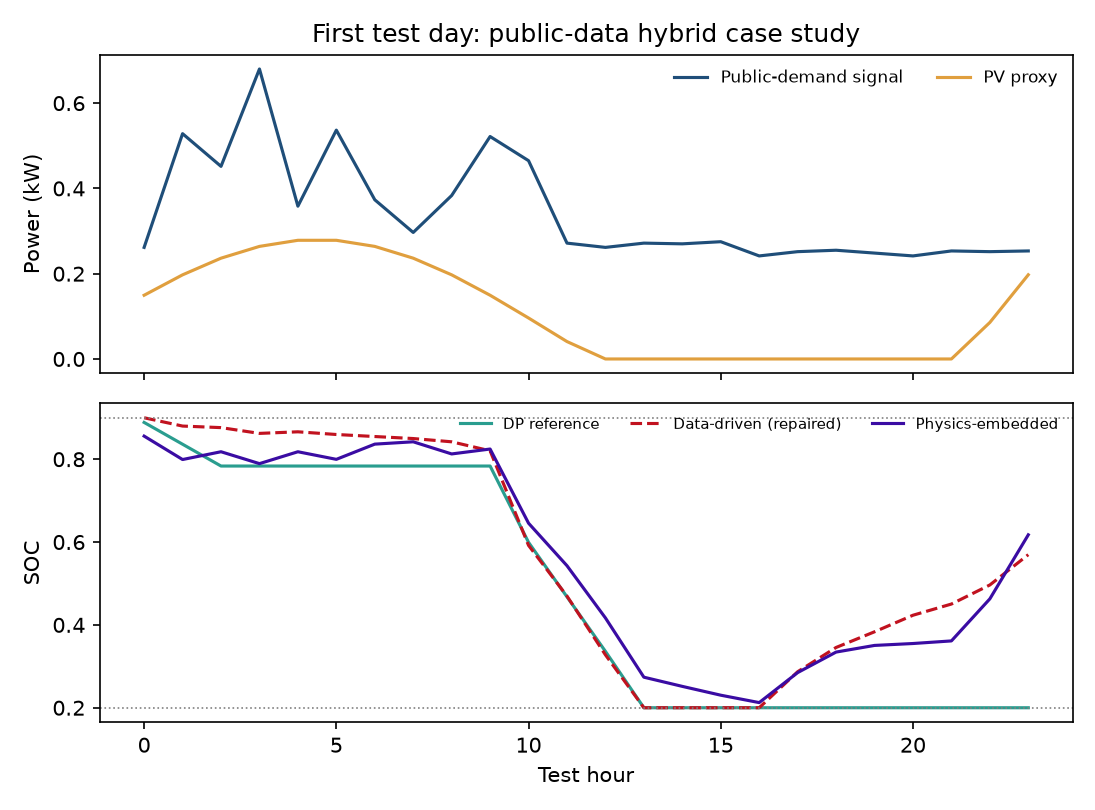
\includegraphics[width=0.92\textwidth]{fig-first-test-day.png}
  \caption{بار و فتوولتائیک مطالعه موردی و وضعیت شارژ کنترل‌کننده‌ها در نخستین روز آزمون}
  \label{fig:first-test-day}
\end{figure}

\begin{figure}[H]
  \centering
  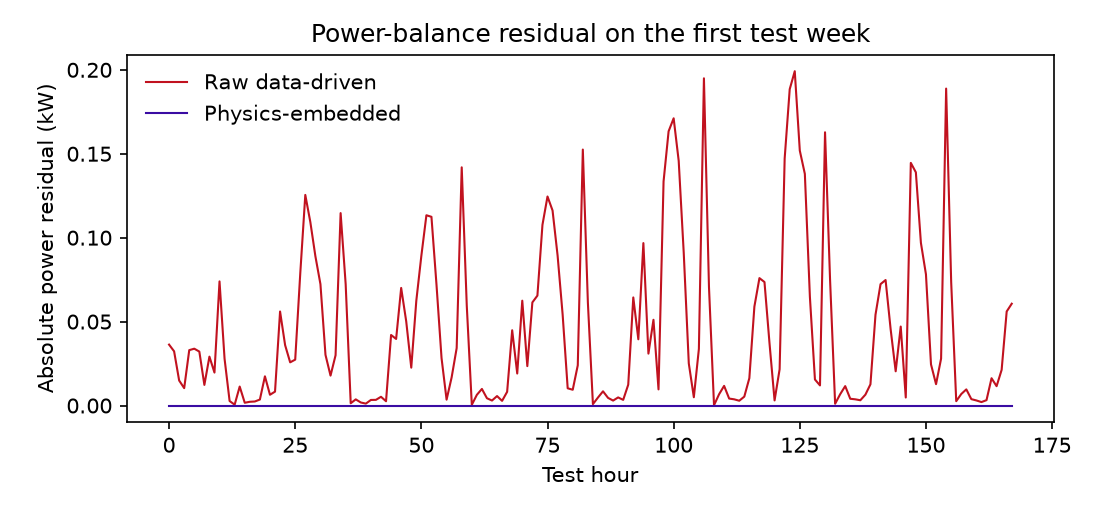
\includegraphics[width=0.92\textwidth]{fig-power-residual.png}
  \caption{قدر مطلق باقیمانده توازن توان در هفته نخست آزمون}
  \label{fig:power-residual}
\end{figure}

\section{هزینه اجرایی}
هزینه کل افق آزمون ۶۵۹ ساعته در جدول~\ref{tab:operating-cost} آمده است. هزینه مدل داده‌محور فقط پس از نگاشت ایمنی محاسبه شده تا نقض قید خام پاداش اقتصادی نگیرد. شبکه فیزیک‌تعبیه‌شده با هزینه $42{.}418\pm 0{.}511$ حدود $6{.}2$ درصد از حالت بدون باتری ارزان‌تر و به‌طور میانگین $2{.}8$ درصد از مرجع برنامه‌ریزی پویا گران‌تر است. هزینه آن با مدل داده‌محور ترمیم‌شده ($42{.}234\pm 0{.}318$) قابل مقایسه است و میانگین ترمیم‌شده اندکی کمتر است. با همپوشانی انحراف معیار پنج بذر، این اختلاف از نظر توصیفی قاطع نیست و آزمون فرض جداگانه‌ای گزارش نشده است. پس امکان‌پذیری تضمین‌شده به معنی رسیدن خودکار به برنامه بهینه افق کامل نیست. شکل~\ref{fig:daily-cost} میانگین هزینه روزانه برنامه‌های قابل اجرا را نشان می‌دهد.

زمان اجرا در محیط بایگانی‌شده آزمایش اندازه‌گیری شد: پردازنده شصت‌وچهاربیتی که مدل دقیق آن در آن محیط آشکار نبود، مفسر پایتون $3{.}11{.}2$ و کتابخانه محاسباتی نام‌پای $2{.}4{.}6$. حل یک‌باره مرجع برنامه‌ریزی پویا برای افق کامل ۳۲۸۹ گام $0{.}540$ ثانیه طول کشید. زمان یک گام کنترل‌کننده، شامل گذر پیش‌رو در شبکه $32\times 32$، نگاشت تانژانت هیپربولیک و لایه تحلیلی، پس از ۱۰۰۰ فراخوانی گرم‌سازی و در ۱۰ تکرار ۱۰۰۰۰تایی برابر $21{.}468\pm 0{.}402$ میکروثانیه بود. این اعداد با فرمان \lr{python code/benchmark\_runtime.py} بازتولید می‌شوند. برای سخت‌افزار دیگر باید نوع پردازنده یا شتاب‌دهنده، میانگین، انحراف معیار و شمار فراخوانی‌ها جداگانه ثبت شود.

\begin{table}[H]
  \centering
  \caption{هزینه اجرایی افق آزمون؛ واحد پولی مفروض}
  \label{tab:operating-cost}
  \begin{tabular}{lcc}
    \toprule
    مدل & هزینه کل آزمون & فاصله از مرجع پویا (درصد) \\
    \midrule
    مرجع پویا & $41{.}252$ & $0$ \\
    بدون باتری & $45{.}233$ & $9{.}7$ \\
    داده‌محور با نگاشت ایمنی پس‌پردازشی & $42{.}234\pm 0{.}318$ & $2{.}4\pm 0{.}8$ \\
    فیزیک‌تعبیه‌شده & $42{.}418\pm 0{.}511$ & $2{.}8\pm 1{.}2$ \\
    \bottomrule
  \end{tabular}
\end{table}

\begin{figure}[H]
  \centering
  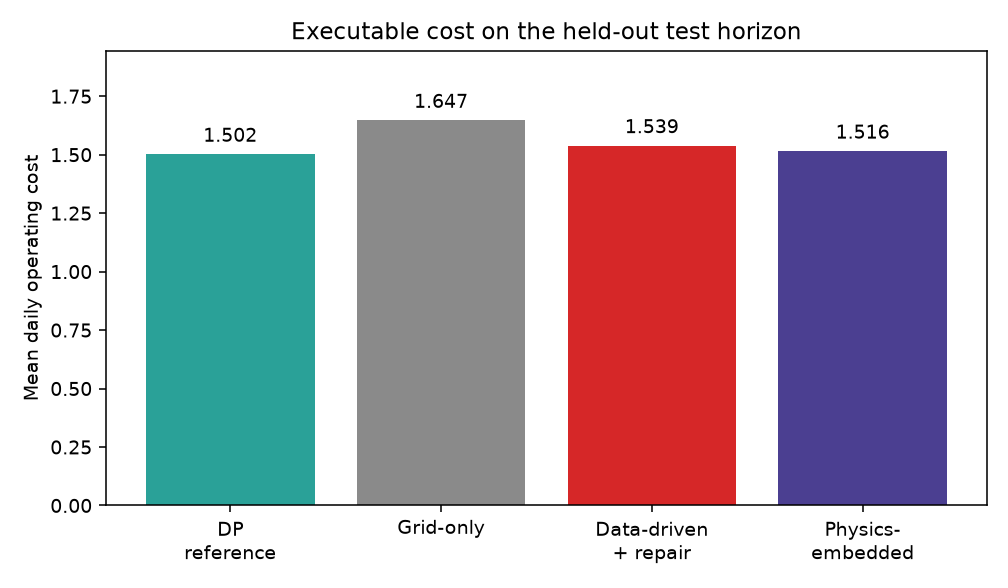
\includegraphics[width=0.78\textwidth]{fig-daily-cost.png}
  \caption{میانگین هزینه روزانه برنامه‌های قابل اجرا روی افق آزمون}
  \label{fig:daily-cost}
\end{figure}

\section{تفسیر و محدودیت‌ها}
نتیجه اصلی فقط کاهش خطای میانگین نیست. شبکه فیزیک‌تعبیه‌شده با اندکی افزایش خطای تقلید نسبت به مدل آزاد، برنامه‌هایی می‌سازد که از نظر قیود تعریف‌شده همواره قابل اجرا هستند. مدل آزاد برای استفاده عملی به تعمیر پس‌پردازشی نیاز دارد. این موازنه با ادبیات قید سخت سازگار است: محدود کردن فضای خروجی آزادی تقریب را کم می‌کند، اما اعتماد فیزیکی را بالا می‌برد \pcite{lu2021hardconstraints,chen2024hardlinear}.

محدودیت‌ها نیز روشن‌اند. داده ترکیبی است و تابش فتوولتائیک ساعتی در همان خانه اندازه‌گیری نشده است. ورودی‌های یک و سه ساعت آینده و افق مرجع برنامه‌ریزی پویا با آینده‌نگری کامل‌اند. تبادل شبکه نامحدود فرض شده؛ اگر سقف اتصال باشد، لایه سخت باید فرمان باتری را با بازه مجاز $P_{\mathrm{G}}$ سازگار کند. مدل باتری دما، پیری، وابستگی بازده به توان و دینامیک مبدل را ندارد. نگاه‌به‌جلو در چند نمونه پایانی هر افراز می‌تواند سیگنال برون‌زاد افراز بعدی را ببیند؛ این نشت مرزی محدود است و برچسب آزمون در آموزش نیست. در آموزش $s$ از مسیر مرجع است و در آزمون بازگشتی از خود مدل؛ این ناهماهنگی توزیع هم در شکاف هزینه نقش دارد. بنابراین این گزارش برتری صنعتی یا عملکرد با خطای پیش‌بینی را نشان نمی‌دهد.

آنچه در ادامه می‌آید فقط پروتکل پیشنهادی کارهای آینده است، نه نتیجه آزمایش‌شده. در یک \textbf{جاروب حساسیت} هر بار فقط یکی از $P_{\max}$، $E_{\max}$، بازده‌ها، $\kappa$ و فاصله قیمت خرید و فروش، روی شبکه‌ای از پیش ثبت‌شده، عوض شود؛ برای هر حالت مرجع و پنج بذر دوباره اجرا شوند و هزینه، فاصله از برنامه‌ریزی پویا و نقض‌ها گزارش گردند. سپس ورودی‌های نگاه‌به‌جلو $t+1$ و $t+3$ جداگانه و هم‌زمان حذف شوند؛ پیش‌بینی‌ها با خطاهای کالیبره‌شده جایگزین گردند؛ و روزهای خارج از توزیع، برحسب فصل یا صدک بار، کنار گذاشته و فقط برای آزمون به کار روند. منحنی آموزش باید زیان آموزش و اعتبارسنجی هر بذر و نقطه توقف را نشان دهد. \textbf{تحلیل رژیمی} نیز، پیش از دیدن نتیجه، ساعت‌های نزدیک $s_{\min}$ و ساعت‌های تغییر دوره تعرفه را تعریف کند و میانگین قدر مطلق خطا، هزینه و نرخ نقض را جداگانه گزارش نماید.

\chapter{جمع‌بندی و پیشنهادها}
\label{chap:conclusion}

\section{جمع‌بندی}
این گزارش چارچوبی اولیه برای کاربرد شبکه‌های عصبی فیزیک‌آگاه در مدیریت انرژی ریزشبکه ارائه کرد. مسئله مدیریت انرژی مجموعه‌ای از تصمیم‌های به‌هم‌پیوسته درباره تأمین بار، تولید تجدیدپذیر، باتری و تبادل توان با شبکه اصلی است. در چنین مسئله‌ای، دقت داده‌ای به‌تنهایی کافی نیست و خروجی مدل باید با توازن توان و محدودیت‌های تجهیزات سازگار باشد.

ایده اصلی شبکه فیزیک‌آگاه آن است که قوانین حاکم بر سامانه در تابع هزینه آموزش وارد شوند. این ایده از چارچوب عمومی رئیسی و همکاران برای حل و شناسایی معادلات دیفرانسیل الهام گرفته است \pcite{raissi2019pinns}. برای صورت‌بندی بخش ریزشبکه نیز از ساختار مدیریت انرژی، ذخیره‌ساز و تبادل توان در پژوهش اولادجو و فولی استفاده شد \pcite{oladejo2019microgrid}. بر این اساس، مؤلفه‌های توازن توان، پویایی وضعیت شارژ، حدود بهره‌برداری و هدف اقتصادی در یک تابع هزینه ترکیبی قرار گرفتند.

چارچوب ارائه‌شده یک طرح قابل پیاده‌سازی است و درباره برتری عددی مدل ادعایی ندارد. نتیجه‌گیری تجربی تنها پس از آماده‌سازی داده، اجرای کد و مقایسه منصفانه مدل فیزیک‌آگاه با مدل‌های پایه امکان‌پذیر است. این تفکیک میان طراحی روش و نتیجه تجربی برای حفظ اعتبار علمی پروژه ضروری است.

\section{پیشنهادها برای ادامه کار}
مسیرهای زیر می‌توانند در ادامه پروژه بررسی شوند:
\begin{enumerate}
  \item تکمیل مجموعه‌داده یا ساخت شبیه‌ساز معتبر برای ریزشبکه؛
  \item بررسی راهبردهای مختلف برای وزن‌دهی مؤلفه‌های تابع هزینه؛
  \item مقایسه شبکه فیزیک‌آگاه با شبکه عصبی صرفاً داده‌محور و یک روش بهینه‌سازی کلاسیک؛
  \item افزودن عدم قطعیت تولید خورشیدی، قیمت و بار؛
  \item استفاده از قید سخت به جای جریمه نرم برای متغیرهای حساس؛
  \item توسعه مدل برای حالت جزیره‌ای یا چند ریزشبکه متصل؛
  \item ترکیب نظریه بازی با مدل فیزیک‌آگاه برای تخصیص منصفانه سود؛
  \item بررسی مدل‌های زمانی مانند شبکه بازگشتی یا ترنسفورمر فیزیک‌آگاه؛
  \item ارزیابی زمان استنتاج برای کاربردهای برخط؛
  \item انتشار کد و تنظیمات آزمایش برای افزایش تکرارپذیری.
\end{enumerate}

\section{سخن پایانی}
شبکه‌های عصبی فیزیک‌آگاه پلی میان مدل‌سازی ریاضی و یادگیری از داده ایجاد می‌کنند. ارزش این رویکرد در مسئله ریزشبکه زمانی روشن می‌شود که هم معیارهای یادگیری و هم قوانین فیزیکی با دقت تعریف و ارزیابی شوند. نسخه نهایی پروژه باید این چارچوب را با داده و آزمایش واقعی تکمیل کند و محدودیت‌های مشاهده‌شده را نیز در کنار نقاط قوت گزارش دهد.


% پیوست اختیاری
\ifIncludeAppendix
  \appendix
  \chapter{نمونه دستورات پرکاربرد LaTeX}
\label{app:latex-examples}

این پیوست به‌طور پیش‌فرض غیرفعال است. برای نمایش آن، مقدار
\lr{\textbackslash IncludeAppendixtrue}
را در فایل \lr{config/metadata.tex} قرار دهید.

\section{ارجاع به منبع}
برای ارجاع عددی از دستور زیر استفاده کنید:
\begin{latin}
\begin{verbatim}
\cite{raissi2019pinns}
\end{verbatim}
\end{latin}

\section{درج شکل}
\begin{latin}
\begin{verbatim}
\begin{figure}[H]
  \centering
  \includegraphics[width=0.75\textwidth]{my-figure.pdf}
  \caption{Figure caption}
  \label{fig:my-figure}
\end{figure}
\end{verbatim}
\end{latin}

\section{درج جدول}
\begin{latin}
\begin{verbatim}
\begin{table}[H]
  \centering
  \caption{Table caption}
  \label{tab:my-table}
  \begin{tabular}{lc}
    \toprule
    Parameter & Value \\
    \midrule
    Width & 64 \\
    \bottomrule
  \end{tabular}
\end{table}
\end{verbatim}
\end{latin}

\fi

% منابع
\cleardoublepage
\phantomsection
\chapter*{منابع}
\addcontentsline{toc}{chapter}{منابع}
\begin{latin}
\sloppy
\hbadness=2500 % عنوان‌های طولانی منابع IEEE هشدار کم‌اهمیت ایجاد نکنند.
\printbibliography[heading=none]
\end{latin}

% صفحات انگلیسی پایانی، مطابق ترتیب دستورالعمل دانشگاه
\ifIncludeEnglishPages
  \cleardoublepage
  \hypersetup{pageanchor=false}
  \pagenumbering{gobble}
  \thispagestyle{empty}
\begin{latin}
\sloppy
\hbadness=2500 % کنترل هشدارهای کم‌اهمیت ناشی از واژه‌های مرکب انگلیسی
% عنوان این صفحه عمداً با \chapter* ساخته نشده است؛ زیرا قلم فارسی B Titr
% حروف لاتین ندارد و در آن حالت واژه Abstract به‌صورت مربع نمایش داده می‌شود.
{\bfseries\fontsize{20pt}{28pt}\selectfont Abstract\par}
\vspace{1.1cm}

Energy management of a grid-connected microgrid must account for operating cost as well as battery constraints. A neural network that independently predicts grid exchange, charge, discharge and state of charge can achieve a small approximation error while producing an infeasible command, such as simultaneous charging and discharging or an out-of-range state of charge. This study develops a physics-embedded neural network that learns only a signed battery command. A parameter-free analytical output layer derives charge, discharge, next state of charge and grid power so that power balance, state-of-charge bounds, battery power limits, non-negativity and charge-discharge exclusivity hold by construction.

The case study contains 3,289 hourly records over the processed interval from 17:00 on 11 January to 17:00 on 27 May 2016. The calendar follows a public appliance data set; because the UCI and NASA POWER hosts were unreachable in this run, load and PV were filled with a documented residential shape and a solar-altitude envelope at Stambruges, while the PV rating, background load and tariff remain stated engineering assumptions. A constrained dynamic-programming schedule provides a reference. An unconstrained data-driven MLP and the physics-embedded MLP are trained with a chronological 60/20/20 split and five random seeds, then evaluated in autoregressive test rollouts.

By construction of the output layer, the physics-embedded model has a zero power-balance residual and zero rate for every defined constraint violation in floating-point evaluation. Although the raw data-driven model had a lower MSE, it produced about 11.4 percent state-of-charge violations and 35.4 percent simultaneous charge-discharge commands. The physics-embedded controller cost $42{.}418 \pm 0{.}511$, i.e., 6.2 percent less than grid-only operation and 2.8 percent more than the dynamic-programming reference. Its cost was comparable to the repaired data-driven model ($42{.}234 \pm 0{.}318$), whose mean was slightly lower, but the difference is not conclusive given the spread across five seeds, and no formal hypothesis test is reported. Zero violations are a design property, not a statistical discovery. The finding is limited to this hybrid public-data case study and is not claimed to generalize to field or industrial operation.

\vspace{0.6cm}
\noindent\textbf{Keywords:} \KeywordsEn
\end{latin}

  \thispagestyle{empty}
\begin{latin}
\begin{center}
  
\includegraphics[width=3.2cm]{logo.pdf}

  \vspace{0.5cm}
  {\bfseries\fontsize{13pt}{18pt}\selectfont
  \UniversityNameEn\\[0.25cm]
  \FacultyNameEn\\[0.15cm]
  \DepartmentNameEn}

  \vfill
  {\bfseries\fontsize{15pt}{21pt}\selectfont
  A \DegreeNameEn{} Project in \FieldNameEn}

  \vspace{0.7cm}
  {\bfseries\fontsize{19pt}{27pt}\selectfont
  \ProjectTitleEn}

  \vfill
  {\bfseries \SupervisorLabelEn}\\[0.25cm]
  \SupervisorNameEn

  \ifdefempty{\AdvisorNameEn}{}{%
    \vspace{0.5cm}
    {\bfseries \AdvisorLabelEn}\\[0.25cm]
    \AdvisorNameEn
  }

  \vfill
  {\bfseries \AuthorLabelEn}\\[0.25cm]
  \StudentNameEn\\[0.15cm]
  \StudentIdLabelEn: \StudentNumber

  \vfill
  {\bfseries \DefenseDateEn}
\end{center}
\end{latin}

\fi

\end{document}
